\subsection{Descripci\'on del Escenario}
	\par En este escenario se monitorearon los paquetes ARP de la red Wi-Fi de acceso publico de un local de comida rápida en una zona muy concurrida de la ciudad de Buenos Aires.[Starbucks en Av. Callao]

	\par A la hora del analisis, mi posición es de completo desconocimiento sobre la naturaleza de la red, quienes intervienen en la misma y el accionar de los usuarios en ella.
    
	\par Se espera que en general las conexiones de los diversos dispositivos de la gente que concurre al local sea de algunos pocos minutos y busque simplemente acceder a internet, por lo cual se espera que la principal conmutación se de entre las IPs de estos dispositivos y el gateway.



\subsection{An\'alisis de datos obtenidos}
	\par La captura fue de 45 minutos y se enviaron 947 paquetes, el grafo dirigido de conexiones que se obtuvo fue el siguiente:

 %[-Grafo-]
 
 \begin{figure}[H]
		\centering
		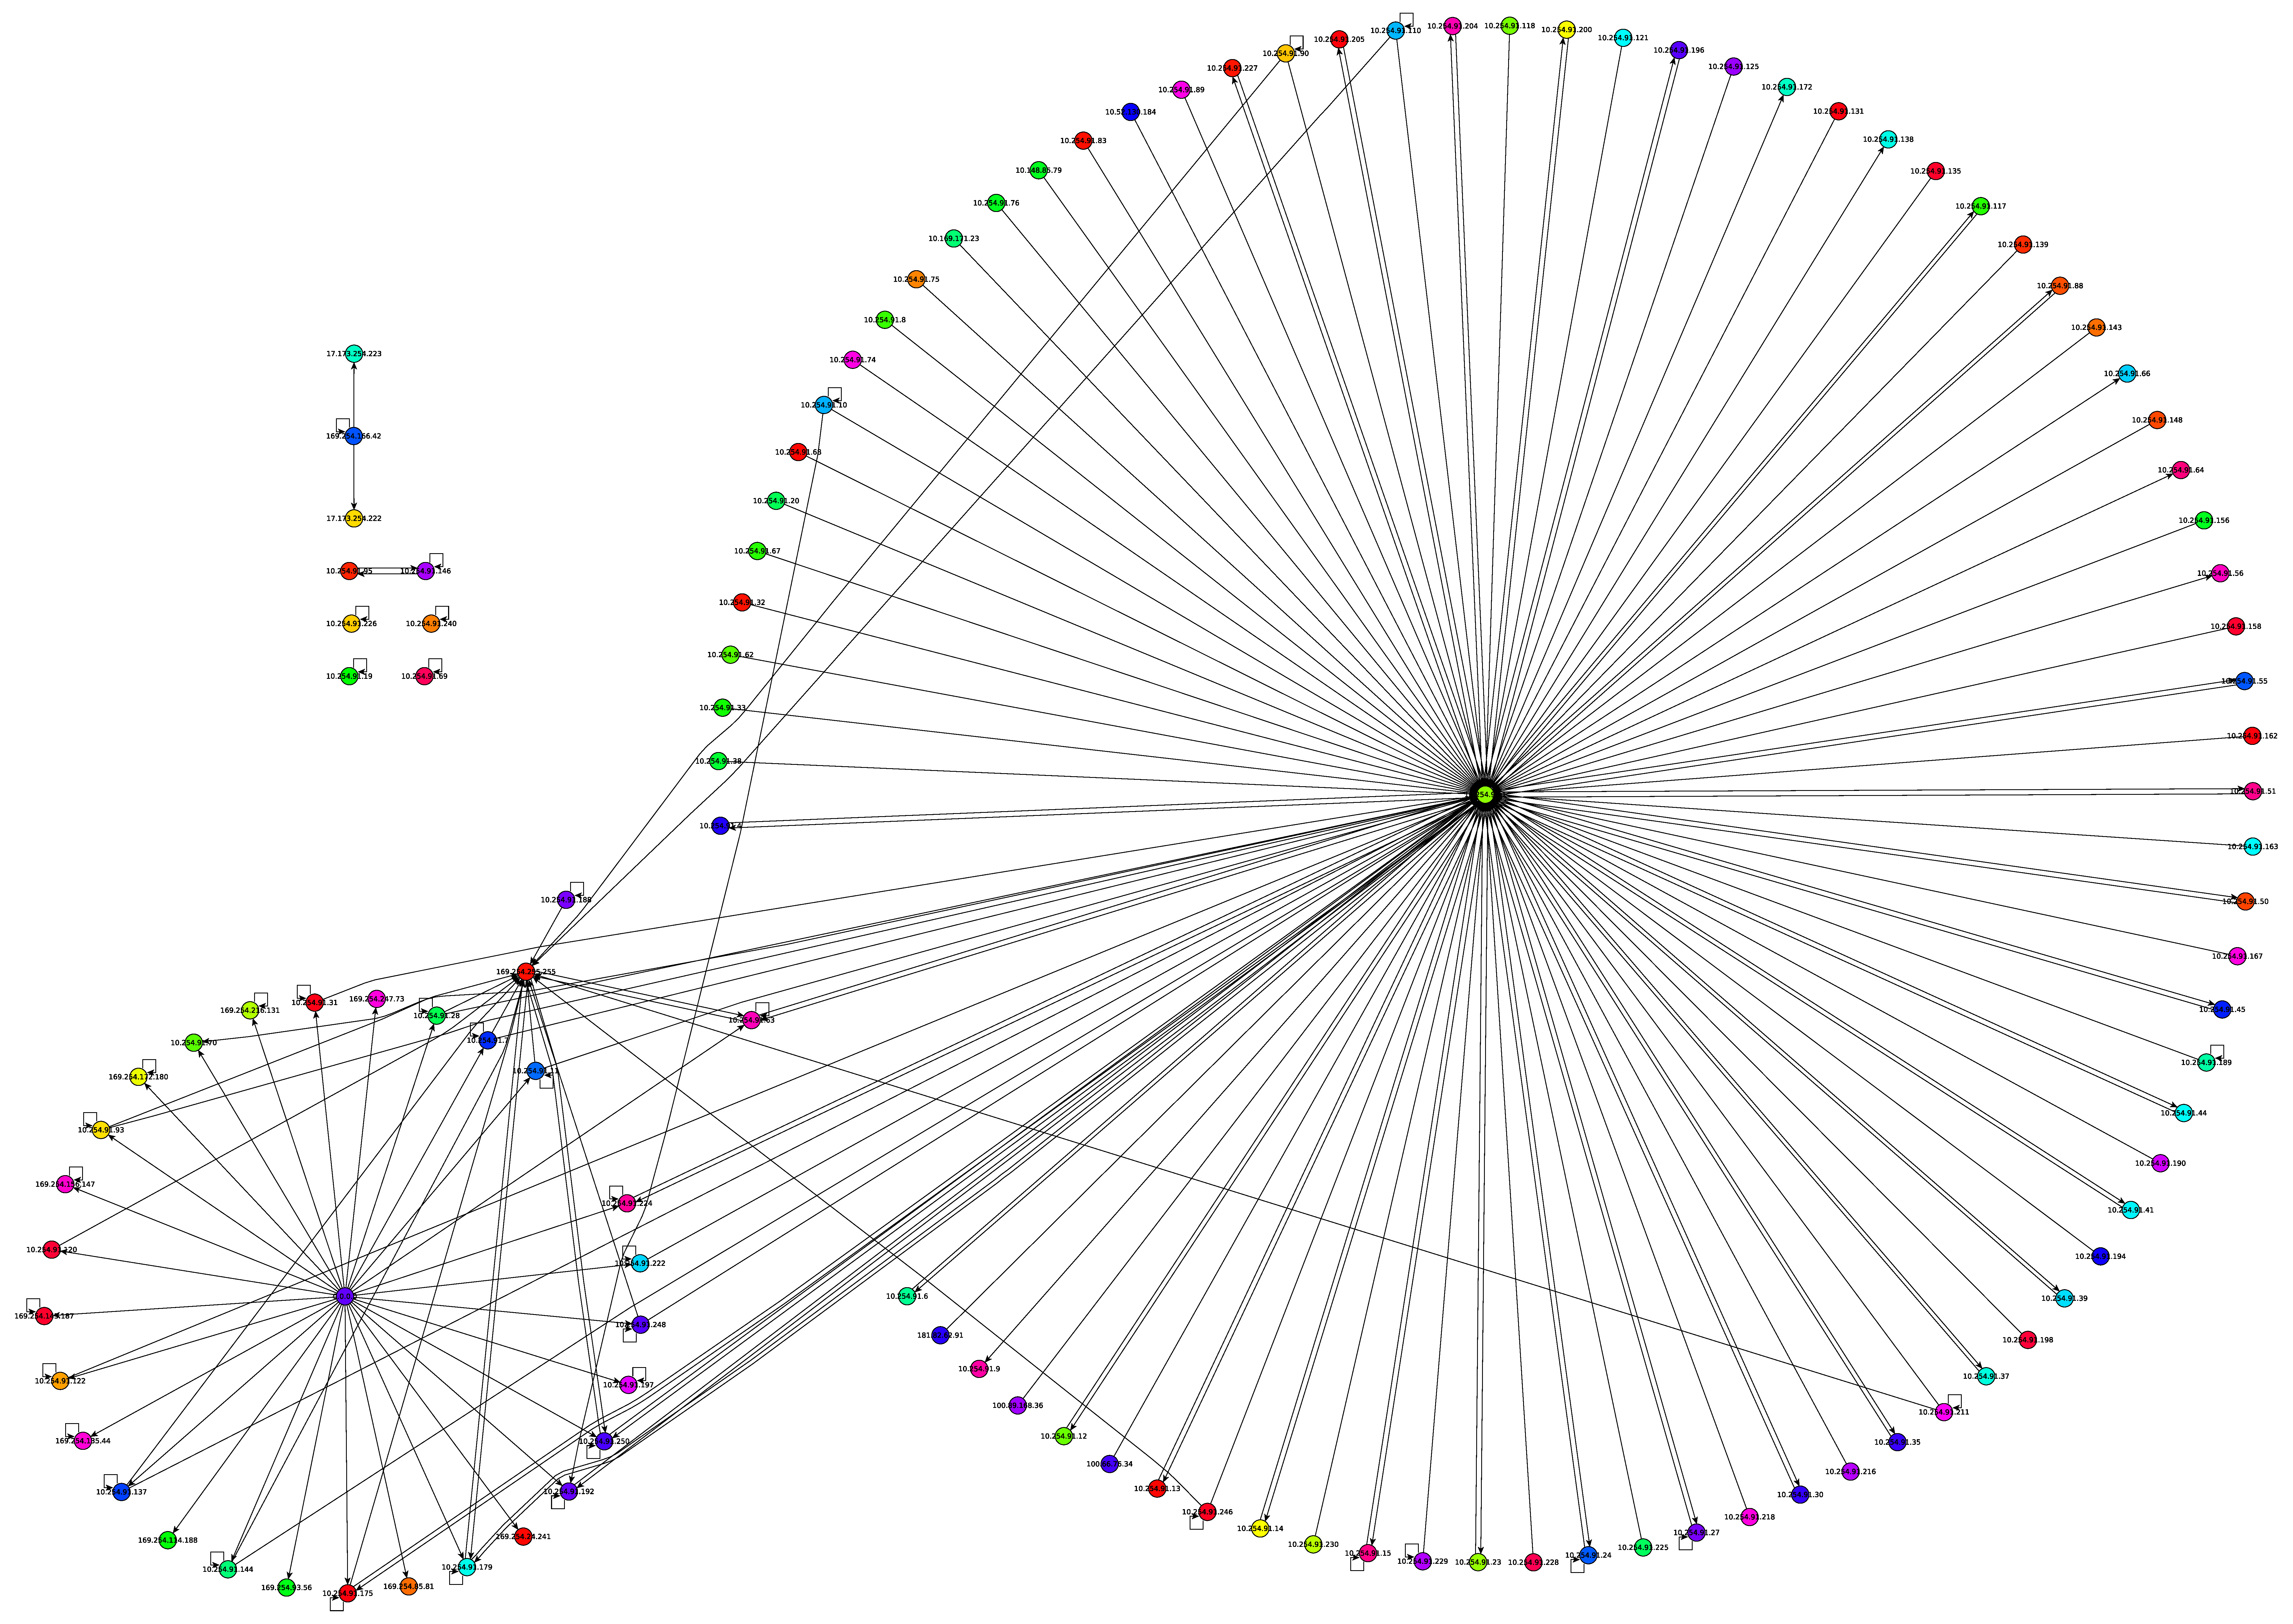
\includegraphics[width=0.5\textwidth]{img/graph/escenario_3/starbucks2.eps}
		\caption{Grafo de la red del Escenario 3}
		\label{fig:grafo_escenario3}
	\end{figure}

	\par Como el grafo es de gran tamaño vamos a considerar subgrafos donde se encuentran nodos interesantes para el analisis.

	\par Hay dos direcciones involucradas en gran parte del tráfico de paquetes, la 10.254.91.1 que  recibe y envia hacia una gran cantidad de IPs y la 169.254.255.255 que principalmente es destino.

	\par La primera se comporta como el gateaway, interactua con la mayoria de las IPs y es la más activa de la red.  

%[-Zoom a IP 10.254.91.1-]

\begin{figure}[H]
		\centering
		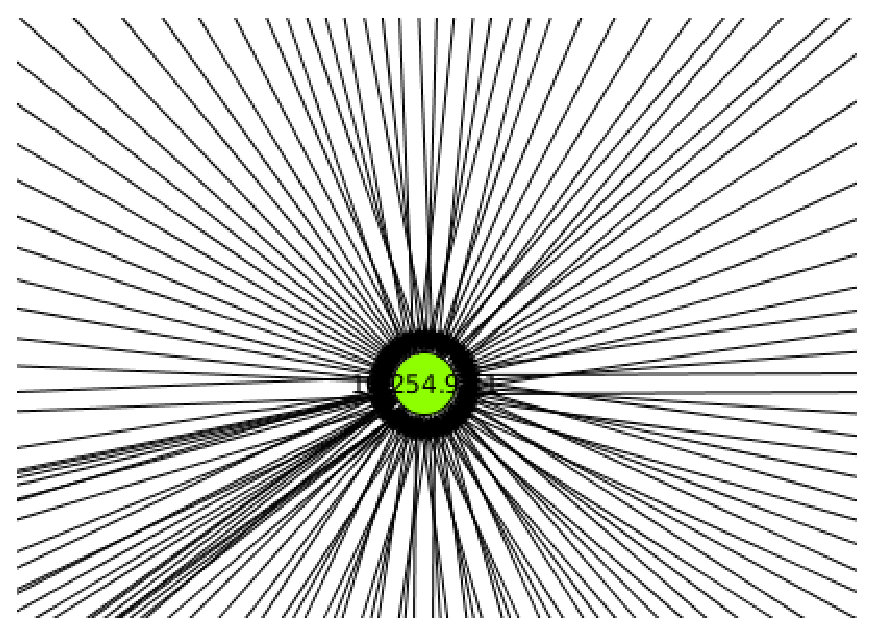
\includegraphics[width=0.5\textwidth]{img/graph/escenario_3/10254.eps}
		\caption{Ampliación en la cercan\'ia a 10.254.91.1}
		\label{fig:grafo_escenario3}
	\end{figure}


	\par La segunda es una direccion reservada  a la que los dispositivos envian paquetes ARP al no encontrar el servidor DHCP ya sea por recien conectarse o perder la ruta hacia el , el dispositivo se asigna una direccion para acceder y comunicarse a la red que usará hasta que se le asigne una IP mediante DHCP. 

%[-Vecindad de la IP 169.254.255.255-]

	\par Tambien se destaca que hay varias who-has con origen 0.0.0.0, esto se da porque al conectarse a la red ciertos dispositvo envian broadcast para ser detectados por el servidor y les asigne una IP, esto termina resultando en un paquete ARP con la IP asignada.

%[-Vecindad de la IP 0.0.0.0-]

	\par El resto de las direcciones se encuentran en el rango 10.254/16, lo cual es completamente razonable y 169.254/16 que es un caso más interesante, estas direcciones son conocidas como Link-local addresses, son direcciones reservadas asignadas en Windows cuando no puede establecer contacto con el servidor DHCP y se genera su propia IP mediante el direccionamiento conocido como APIPA.

	\par El sistema operativo intentará constantemente conectarse con DHCP y recibir una IP válida, mientras tanto los hosts con estas direcciones pueden comunicarse entre si dentro de la red, pero no con ninguno externo a la red local.

	\par Algunas otras caracteristicas del grafo son:

\begin{itemize}

\item Nodos Aislados:

	\par En el grafo se presentan nodos que podemos definir como aislados dado que no se conectan con el gateway 10.254.91.1.
Estos dispositivos se comunican entre sí, con si mismos, o con nadie como es el caso de 17.173.254.223 que no envia paquetes.

	\par  Como es minimamente necesario que envien un paquete a 10.254.91.1 apenas ingresan a la red, nos hace suponer que el host se encontraba conectado a la red antes de hacer el análisis y de esta forma obtuvieron su direccion.  

%[-Subgrafo con nodos aislados-]

\item Nodos Reflexivos:

	\par Podemos destacar nodos que envian paquetes a si mismos, algunos motivos por los que puede suceder esto es para actualizar la tabla ARP, para buscar duplicados de la direccion IP o cambios de la direccion MAC.Este envio de paquetes se conoce como Gratuitous ARP.

\end{itemize}
%http://wiki.wireshark.org/Gratuitous_ARP



	\subsubsection{Entrop\'ia}
		\par Entrop\'ia

\subsection{Conclusiones Preliminares}
